\section{Did you ever argue with your parents about clothes or haircuts?}
Not really.
When I was a child the community in which I lived was comprised primarily of Mennonite families.
There were others who were not Mennonite in the community but my school, church and home life was influenced by the Mennonite church and its culture of the mid twentieth century.
I grew up knowing that it was not a good thing to disagree with or talk back to people in authority.
So generally it was difficult as a young person to express ideas and wishes that were not like those of my parents.

In my world, boys got short haircuts and girls grew their hair long and wore it mostly in two braids.
There were a few times that I remember having ribbons put in my hair.
This happened when my two braids were tied up with ribbons into a basket handle.
This was not a regular occurrence and that may have been because it would have taken considerable time to keep ribbons washed and nicely ironed for three girls.
\begin{figure}
\centering
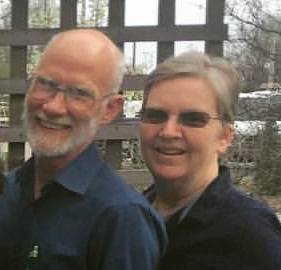
\includegraphics[width=0.45\textwidth]{childhood/8.jpg}
\caption{
One of my last bought dresses before the change to cape dresses.
}
\end{figure}

When I got married I still had long hair so the issue of haircuts was not a problem I took up with my parents.
However, how I worn it was a concern.
The temptation was to get a smaller and smaller covering and try new and more interesting ways to wear my hair.
But the dress rules of Lancaster Mennonite Conference were changing and so my parents no longer had that authority to back them up.
We were allowed to make some changes.

However, the clothing issue had been ongoing.
At nine my mother put me in a dress with a cape, my hair was put in a bun and a covering was put on top of that.
Let's just say I did not like that.
My mother sewed a lot of clothing for her children, primarily the girls.
The fact that I can remember two bought dresses, tells you that I did not have many dresses that my mother did not make.
Once I dressed plain that pretty much sealed the deal, my mother made the dresses I worn.
Some may have been hand me downs but I don't really remember those.
\begin{figure}
\centering
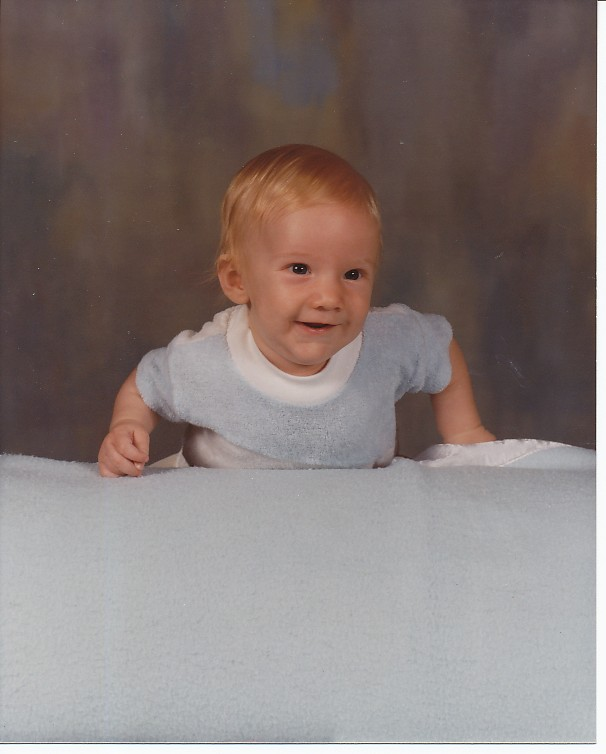
\includegraphics[width=0.6\textwidth]{childhood/9.jpg}
\caption{
Note my cape dress.
}
\end{figure}

I do remember as a chubby pre-adolescent trying to stand still as my mother fit different parts of the dress on me.
There were often pins that stuck me.
My mother did not intend for that to happen but it contributed to me feeling uncooperative with the whole process of dress making.
It was high school until I began to sew some of my own clothing.
We were allowed to wear a skirt like culottes and blouse for physical education.
These were store bought.

My mother had remarkable patience as she sewed for all of her girls but not likely all at the same time.
The cape dress became a thing of the past for me my senior year in high school when LMS decide to drop that clothing requirement for girls.
For graduation senior girls were invited to wear a pastel dress to the baccalaureate service and a white dress to the graduation ceremony.
I do (thanks to pictures) remember the white shift style dress with a stand up collar that I wore for graduation day.
\begin{figure}
\centering
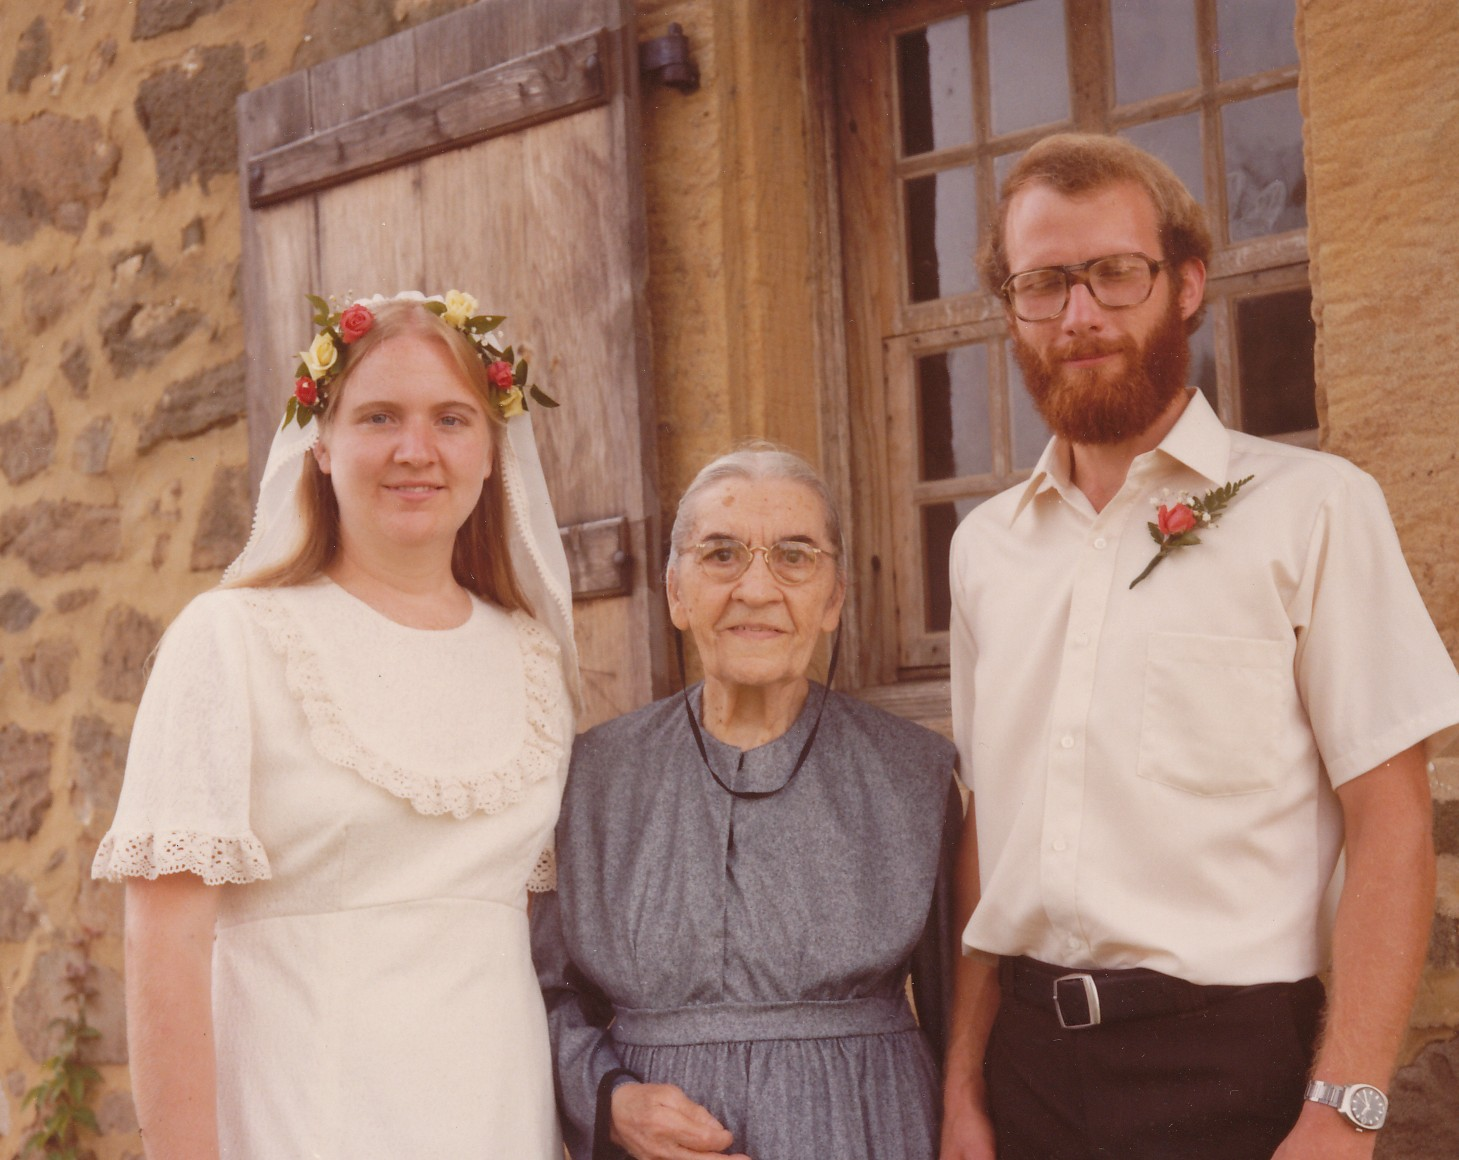
\includegraphics[width=0.6\textwidth]{childhood/10.jpg}
\caption{
White dress for graduation day.
}
\end{figure}
I do not have memories of open and respectful conversations with my parents about our differences about dress and hair.
There were other more verbal siblings who made the attempt to talk with the parents about these issues.
Some were more successful than others.
I have to describe my way of dealing with this conflict as avoidance and when possible going ahead and making my own decisions about dress and hair.
That spilled over into how I dressed my children.
John and I chose to not dress plain and that impacted the kind of clothing we chose for our children.





